\documentclass[conference]{IEEEtran}
\IEEEoverridecommandlockouts
% The preceding line is only needed to identify funding in the first footnote. If that is unneeded, please comment it out.
\usepackage{amsmath,amssymb,amsfonts}
\usepackage{algorithmic}
\usepackage{graphicx}
\usepackage{textcomp}
\usepackage{xcolor}
\def\BibTeX{{\rm B\kern-.05em{\sc i\kern-.025em b}\kern-.08em
    T\kern-.1667em\lower.7ex\hbox{E}\kern-.125emX}}
\usepackage[utf8]{inputenc}
%\usepackage[a4paper, total={6in, 8in}]{geometry}
\usepackage{color}

\usepackage{hyperref}
\usepackage{graphicx}
\usepackage{amsmath}

\usepackage[
backend=biber,
style=numeric,
maxnames = 5,
sorting=ynt
]{biblatex}

\addbibresource{cryptocurrency.bib}

\newcommand{\ari}[1]{\textsf{\color{blue}{[Ari: {#1}]}}}


\begin{document}

\title{Negative-Spread Arbitrage Bots in \\ Decentralized Cryptocurrency Exchanges
\thanks{Identify applicable funding agency here. If none, delete this.}
}

\iffalse
\author{\IEEEauthorblockN{1\textsuperscript{st} Given Name Surname}
\IEEEauthorblockA{\textit{dept. name of organization (of Aff.)} \\
\textit{name of organization (of Aff.)}\\
City, Country \\
email address}
\and
\IEEEauthorblockN{2\textsuperscript{nd} Given Name Surname}
\IEEEauthorblockA{\textit{dept. name of organization (of Aff.)} \\
\textit{name of organization (of Aff.)}\\
City, Country \\
email address}
\and
\IEEEauthorblockN{3\textsuperscript{rd} Given Name Surname}
\IEEEauthorblockA{\textit{dept. name of organization (of Aff.)} \\
\textit{name of organization (of Aff.)}\\
City, Country \\
email address}
\and
\IEEEauthorblockN{4\textsuperscript{th} Given Name Surname}
\IEEEauthorblockA{\textit{dept. name of organization (of Aff.)} \\
\textit{name of organization (of Aff.)}\\
City, Country \\
email address}
\and
\IEEEauthorblockN{5\textsuperscript{th} Given Name Surname}
\IEEEauthorblockA{\textit{dept. name of organization (of Aff.)} \\
\textit{name of organization (of Aff.)}\\
City, Country \\
email address}
\and
\IEEEauthorblockN{6\textsuperscript{th} Given Name Surname}
\IEEEauthorblockA{\textit{dept. name of organization (of Aff.)} \\
\textit{name of organization (of Aff.)}\\
City, Country \\
email address}
}
\fi


\maketitle

\begin{abstract}

Decentralized cryptocurrency exchanges (DEXes) rely on smart contracts to hold customer assets and execute trades. They are widely hailed as a solution to the price manipulation and (sometimes massive) thefts of user funds affecting centralized cryptocurrency exchanges. 

DEXes, however, present their own problem: slow order-matching and trading. High latencies create opportunities for sophisticated traders to exploit ordinary users. As DEXes contain publicly visible data that offers unprecedented visibility into traders' behaviors, however, it is possible to glean insights into such adversarial trading that cannot be obtained from the conventional, closed trading systems of most world markets.

We focus in this paper on
a new problem peculiar to DEXes that we call {\em negative-spread arbitrage}, a phenomenon where sell orders may have prices {\em lower} than those of buy orders. Sophisticated traders, or {\em arbitrageurs}, can buy and sell respectively against such orders in atomic transactions whose success guarantees a profit at ordinary users' expense. 

We study a sophisticated community of arbitrage bots in a popular DEX called EtherDelta. Our work includes insights into the community's evolving, competitive behavior that reveal important, general lessons about DEXes. Among our surprising findings: Arbitrageurs make profits almost equal to those of the exchange (EtherDelta) itself; arbitrageurs sometimes pay transaction fees (gas) higher than their potential profit, a seemingly paradoxical phenomenon supported by economic theory, but never before observed arising organically in the wild; Users' typos are the major source of arbitraging opportunities.  

%Among our surprising findings are: (1) The profit of the leading EtherDelta arbitrageur approaches EtherDelta's total trading-fee profits; (2) This arbitrageur over the period of study successfully frontrun all others using techniques we hypothesize in this paper; (3) Arbitrageurs often pay transaction fees (gas) higher than their potential profit, a seemingly paradoxical phenomenon supported by economic theory, but never before observed arising organically in the wild (to the best of our knowledge); (4) The largest arbitrage opportunities arise due to users' typos. 



\end{abstract}

\section{Introduction [\color{red}{Ari}]}
\label{sec:intro}

Cryptocurrency exchanges today handle more than \$10 billion in trade volume per day. The vast majority of this volume occurs in {\em centralized} exchanges, which hold custody of customer assets and settle trades. At best loosely regulated, centralized exchanges have experienced scandals ranging from high-profile thefts~\cite{} in some cases of hundreds of millions of dollars in cryptocurrency to malfeasance such as price manipulation~\cite{gandal2018price}. 

Incidents like these have prompted the pursuit of an alternative architecture in which the exchange itself runs on a blockchain. This design is known as a {\em decentralized exchange} or DEX.


%Like exchanges for traditional financial assets, they allow parties to perform price discovery and trade assets. These exchanges are 

DEXes eliminate the main hazard of centralized exchanges, theft of funds, by holding assets and executing trades in a smart contract, typically in Ethereum. EtherDelta, created in 2017, is a popular example today. Its lightweight approval process permits rapid listing of new tokens~\cite{EtherDelta-listing:2018}---historically, often the first on any exchange. Other notable emerging DEXes include 0x~\cite{} and Airswap~\cite{}\ari{More? Upcoming Binance, etc.}.
EtherDelta supports trades between Ether, the cryptocurrency in Ethereum, and ERC20 tokens, units of value generated generated by smart contracts (and discussed below).

At first glance, DEXes like EtherDelta seem an ideal exchange design. They appear to provide effective price discovery and fair trading, while doing away with the drawbacks of centralized exchanges. All orders are (ostensibly) published in EtherDelta's order book, and trades are atomically executed by a smart contract and visible on the Ethereum blockchain. Funds cannot be stolen by the exchange operator, because they reside in the smart contract.


Despite their clear benefits, however, DEXes have a serious and fundamental weakness: On-chain, smart-contract-mediated trades are slow. (The average Ethereum block time is roughly 15s at the date of writing~\cite{Etherscan}.) Traders thus often attempt to take orders that have already been taken or cancelled, but appear active due to latency. Worse still, adversaries can {\em front-run} orders, observing them in the mempool (set of unprocessed blockchain transactions) and placing their own orders with higher fees (gas) to ensure that they are mined first. A second problem is that users must cancel orders manually (or at least on the client side): Once an order is placed in the order book, it can be taken by anyone who has recorded it, even if deleted by the exchange.

In this paper, we study a particular problem in EtherDelta that we call {\em negative-spread arbitrage}. We emphasize that our findings, however, extend to other DEXes and also hold important lessons on 

\subsection{Our measurement study}

In Aug.~2017, we observed an anomaly in the EtherDelta order book. It often contains buy orders with {\em higher prices} than sell orders. We refer to this phenomenon as a {\em negative spread}. Well-functioning securities marketplaces typically have only non-negative spreads, thanks to their fast information propagation and efficient trade execution. 

Negative spreads  represent market inefficiency that can be exploited by an {\em arbitrageur}. The arbitrager buys an asset at the lower bid price and sells at the higher asking price.

We estimated that for 10 of the most popular tokens (among the hundreds on EtherDelta), negative-spread trading opportunities cumulatively represented a \$1.6+ million annual potential profit---and yet was at the time unexploited. To alert the community to this innate, general problem in DEXes, which have been growing in popularity, we made the decision to disclose it~\cite{ED-Forbes-article:2017}. Within weeks, a community of arbitrage bots---which we refer to simply as {\em arbitrageurs}---cropped up to take advantage of it in EtherDelta.

This arbitrageur community offers rare, instructive insights into the dynamics of market arbitrage and the techniques used by competing players in decentralized exchanges and other types of marketplaces (e.g., Cryptokitties). As we show, arbitrageurs compete aggressively, some even losing money in the process. The publication of all EtherDelta orders and transactions offers an unusually detailed data set for studying such behaviors. (Conventional exchanges, e.g., the NYSE, publish only summary data.) 

In this paper, we focus on and seek to illuminate the dynamics of negative-spread arbitrage in EtherDelta. We additionally discover some behaviors among arbitrageurs previously only considered in the theory of economics, uncover blockchain-based technical strategies by which some arbitrageurs drive others out of the market, and propose some possible remedies that our research has brought to light.

Our findings shed light on more pervasive systemic issues in DEXes that we highlight toward the end of the paper.

\subsection{Contributions}

In brief, we make the following contributions:

\begin{itemize}
    \item {\em Arbitrageur measurement study:} We study the behavior of the arbitrageur community in EtherDelta, measuring the transaction volume it generates, the distribution of profits across arbitrageurs, and the idiosyncracies and evolution of arbitrageur strategies. 
    \item {\em Proposed remedies:} Based on our results, we propose simple user-interface modifications that would eliminate a majority of negative-spread arbitrage opportunities in DEXes.
    \item {\em Discussion of future risks:} We discuss new, related risks to users arising in other DEXes, including 0x and Airswap.
\end{itemize}


%A second problem is that a DEX is not truly decentralized: The operator facilitates counterparty discovery, e.g., maintains the order book as in EtherDelta. In principle, EtherDelta can front-run orders since it observes them before anyone else does---just as a centralized exchange can.\footnote{It can also delay or suppress orders, of course.}



\section{Background: Cryptocurrency Exchanges and DEXes [\color{red}{Iddo}]}
\label{sec:DEXes}

We focus in this paper on EtherDelta. Other DEXes work similarly. (We highlight some differences in Section~\ref{sec:future_risks}.)

EtherDelta maintains an order book at {\tt etherdelta.com}. Any user may act as a {\em maker}, posting in this order book either a buy or sell order for tokens, priced in Ether, the cryptocurrency in Ethereum. A maker digitally signs her order, which references assets deposited in the EtherDelta contract. A counterparty may act as a {\em taker} by identifying an (ostensibly open) order in the order book, countersigning it, and sending the order to the EtherDelta contract. If the order has not yet been taken or cancelled by its creator, and the taker has adequate assets deposited, the contract executes the trade. In other words, the EtherDelta contract performs a fair exchange of tokens for Ether.  

A trader can exploit a negative-spread pair, as defined above, as follows. The trader sends a transaction through her own smart contract that atomically: (1) Takes the buy order, exchanging $X$ ETH for $Y$ tokens and then (2) Takes the sell order, exchanging the $Y$ tokens for $X'$ ETH. The trader obtains profit $X' - X$, minus gas costs. The only risk to the trader is loss of the transaction fees should the transaction fail. Otherwise, given the atomicity of the operation, her profit is guaranteed. (Of course, variants are possible, e.g., matching multiple orders atomically and taking a sell order followed by a buy order.) 

\section{Arbitrage Bot Design and Arbitrage Strategy}
\subsection{Arbitrage Bot Design}
Typically the arbitrage bots share a common design pattern although implementations varies. We can regard the arbitrage bot as a combination of five parts:(1) The order book that keeps track of the latest off-chain order book of the DEX. (2) The pending transaction pool that maintains the pending transactions on the Ethereum Network. (3) The arbitrage smart contract that help the arbitrageur to take the arbitrage opportunities atomically. (4) The Ethereum node that interacts with the Ethereum blockchain and controls the arbitrage contract. (5) The arbitrage strategy that gathers all the information and decide whether there is a arbitrage opportunity, when to take the opportunity and how high the gas price of the arbitrage transaction etc.


\begin{figure}
  \centering
    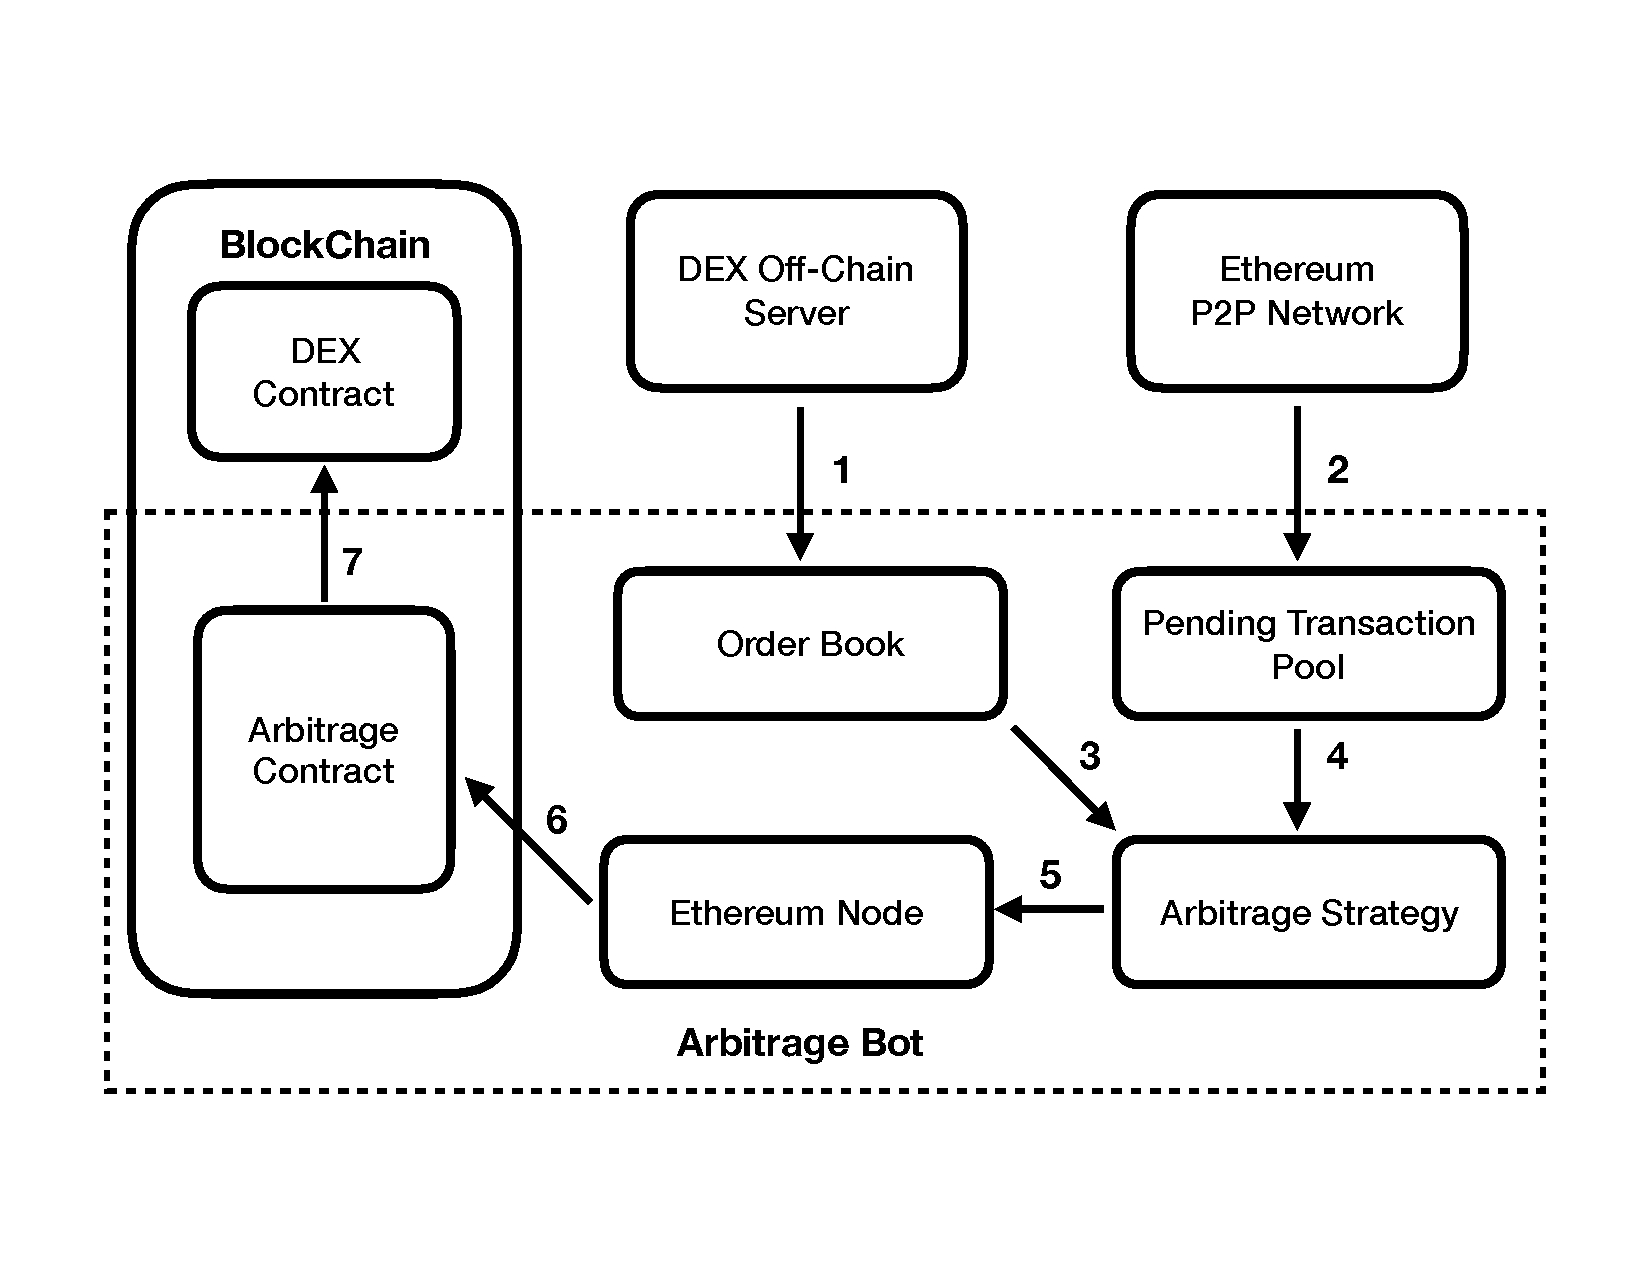
\includegraphics[width=0.5\textwidth]{figures/Arb_Bot_Design.pdf}
  \caption{\textit{The arbitrage bot design: (1) The order book retrieves the newest version of order book from the DEX Off-Chain Server; (2)The pending transaction pool interacts with the Ethereum Peer to Peer Network and updates the status of the transactions; (3) and (4) The arbitrage strategy gather the information provided by the order book and pending transaction pool; (5) The arbitrage strategy control the Ethereum node the send the arbitrage transaction; (6) The Ethereum node send transaction to the arbitrage contract; (7) The arbitrage contract calls the DEX contract to take the orders with atomicity.}}
\end{figure}

\subsection{Arbitrage Strategy}
Some description about the arbitrage strategy that might be useful:
\begin{verbatim}
    https://www.sharelatex.com/8578489683nvnvnxywwhzn
\end{verbatim}

\section{Arbitrageur Profits}


\subsection{Where do arbitrage opportunities come from?}

\subsubsection{Measurement of typos}

\subsubsection{User messages to arbitragers}

\subsection{Summing up}
As we can see, the vast majority of profits accrue to a single arbitrageur, whom we refer to as the {\em dominant arbitrageur (DA)}.

\section{How is the Dominant Arbitrageur Winning?}

\subsection{Is the dominant arbitrageur colluding with miners / EtherDelta?}



\subsection{All-payer auction [\color{red}{Ethan}]}

Include Xueyuan's simple analysis:
For an arbitrage opportunity with profit $profit$.
 Suppose the arbitrageur running algorithm 4 with good network connection has sent the transactions $t_1, t_2 \cdots t_{n}$ in sequence. The corresponding successful gas costs are $c_1, c_2 \cdots c_{n}$ and the failed gas costs are $\lambda c_1,\lambda c_2 \cdots \lambda c_{n}$ where $\lambda \in (0,1)$.
 
 We can assume $c_1 < c_2 < \cdots < c_{n}$ since the arbitrageur will send a new transaction only if there is some competitor send a transaction with a higher price.
 
 If some competitor send a transaction with a higher gas price than $t_{n}$, then the arbitrageur has 2 choices: (1) Do not send a new transaction. (1) Send a new transaction $t_{n+1}$ with a higher gas price $c_{n+1}$, satisfying $c_{n+1} > t_{n}$. 
 
 For the first choice, the worse case is the transaction $t_{n}$ finally fails, so the expected profit for the first choice $E_{1}$ satisfies:
 \[
 	E_1 \geq - \lambda c_{n}
 \]
 For the second choice, the best case is the current transaction succeeded, so the expected profit for the second choice $E_{2}$ satisfies:
 \[
 	E_2 \leq profit - c_{n+1}
 \]

 We can assume arbitrageur with send a new transaction only if when:
\[
	E_2 \geq E_1
\]
So for all $n$, we have:
\begin{align*}
	&profit - c_{n+1} \geq E_2 \geq E_1 \geq - \lambda c_{n} \geq - \lambda c_{n+1} \\
	\Rightarrow & \frac{c_{n+1}}{profit} \leq \frac{1}{1-\lambda}
\end{align*}
Since $\lambda \approx 0.35$, the ratio $c_{n+1}/profit$ is bounded:
\[
	\frac{c_{n+1}}{profit} \leq \frac{1}{1-\lambda} \approx 1.43
\] 

\section{Future Risks}
\label{sec:future_risks}



\pagebreak
\pagebreak
\section*{Questions to Address}

\begin{itemize}
    \item What’s the percentage of arbitrage tx over regular tx (total tx)?
    
    The earliest arbitrage transaction using the contract is: \\ \url{https://etherscan.io/tx/0x95e7e5cdf0130008183b9a178e3ff0175522a30dd4758196ad9eff533fa38257} \\
    The transaction was sent on Jun-28-2017, the arbitrageur sold \href{https://coinmarketcap.com/currencies/amis/}{AMIS} token for some ETH at a higher price, then bought AMIS with some ETH at a lower price. While the maker of the 2 orders is the arbitrageur himself. It seems the arbitrageur was doing some kind of experiment, and the arbitrageur did not continue to do arbitrage. \\
    From block 3900000(2017/6/30) to block 5550000(2018/5/4), there are 2895829 success txs with one or more EtherDelta Trade Event, 80245 (2.77\%) of them are arbitrage txs (transaction that took a pair of orders involving a pair of tokens or ETH). We can see there is a significant increase in the percentage of arbitrage txs after the blog post on Aug. 13th.
    
    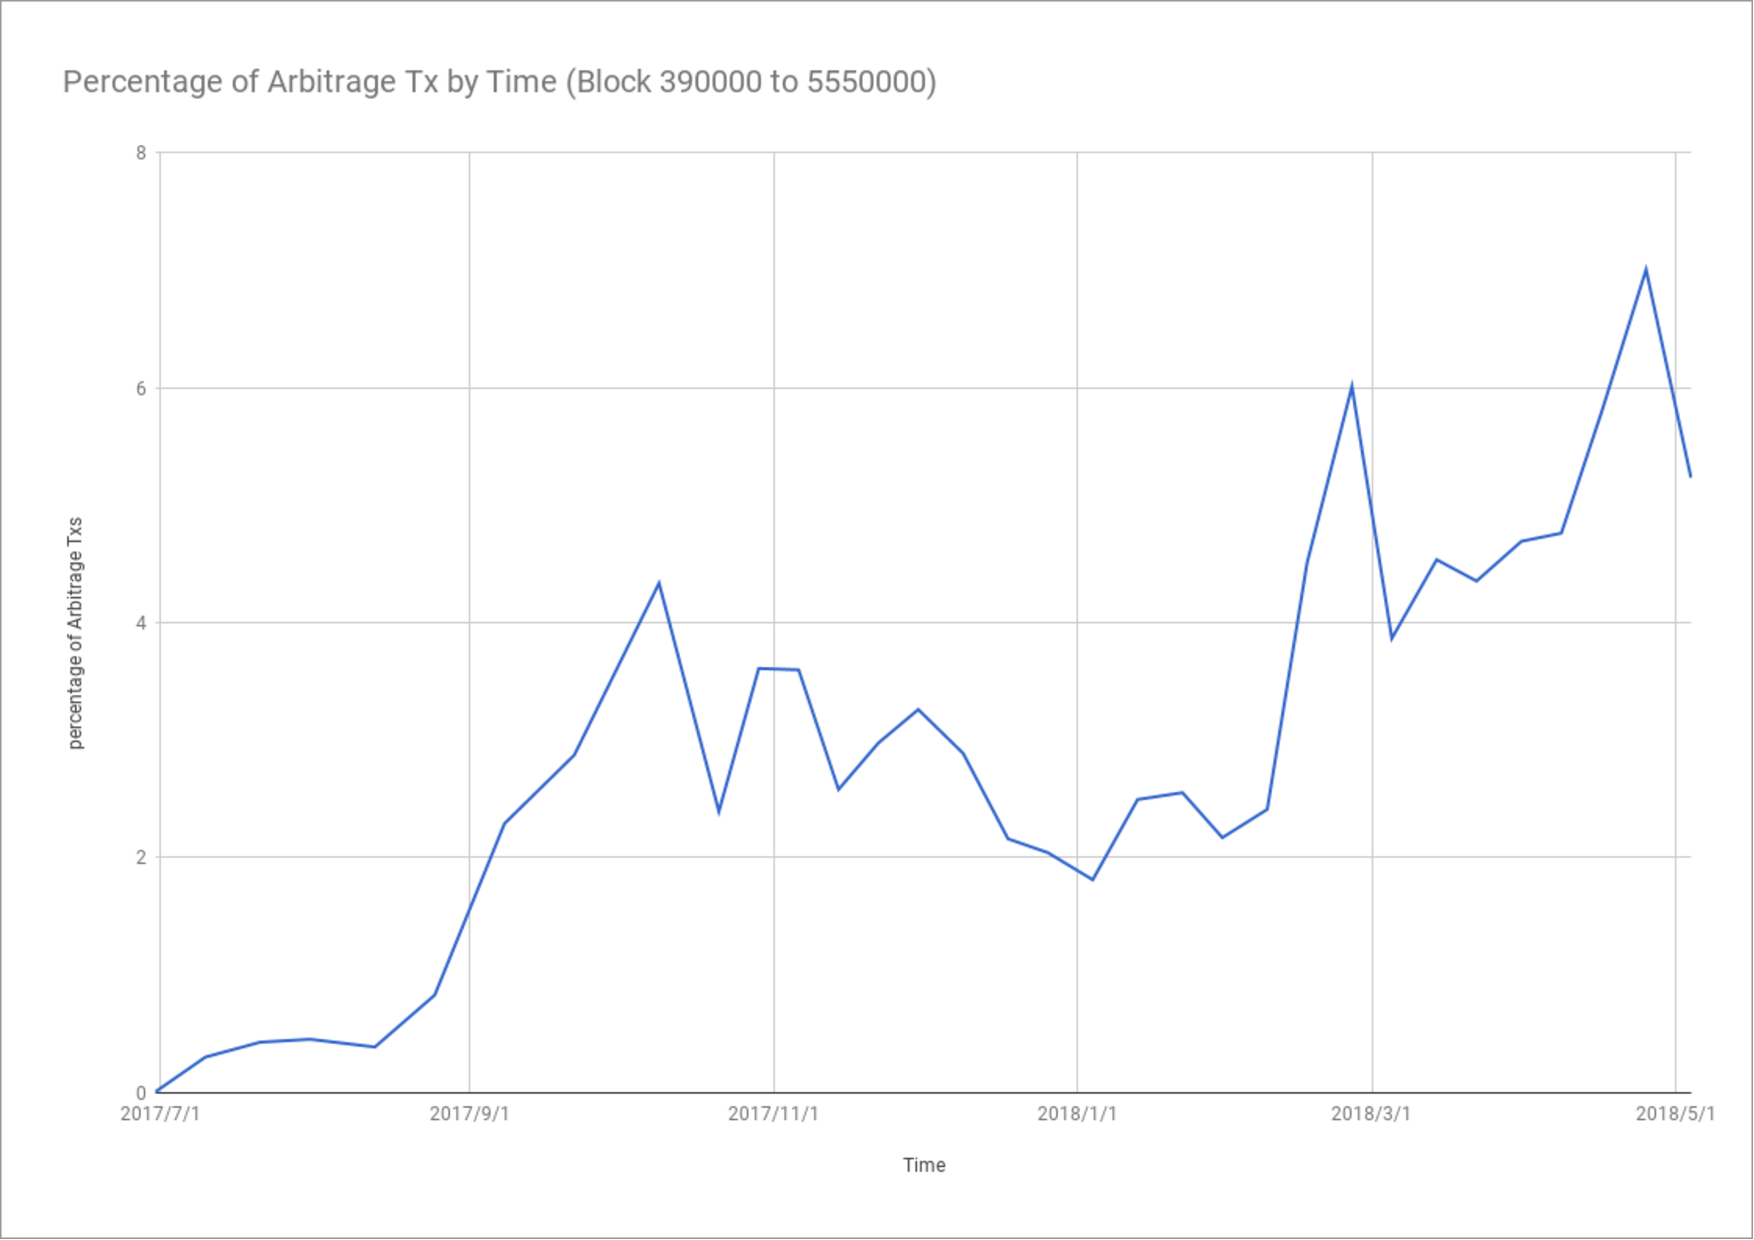
\includegraphics[width=0.5\textwidth]{figures/percentage_by_time.pdf}
    
    \item What’s the relationship between the volume of arbitrage opportunities and gas price?
    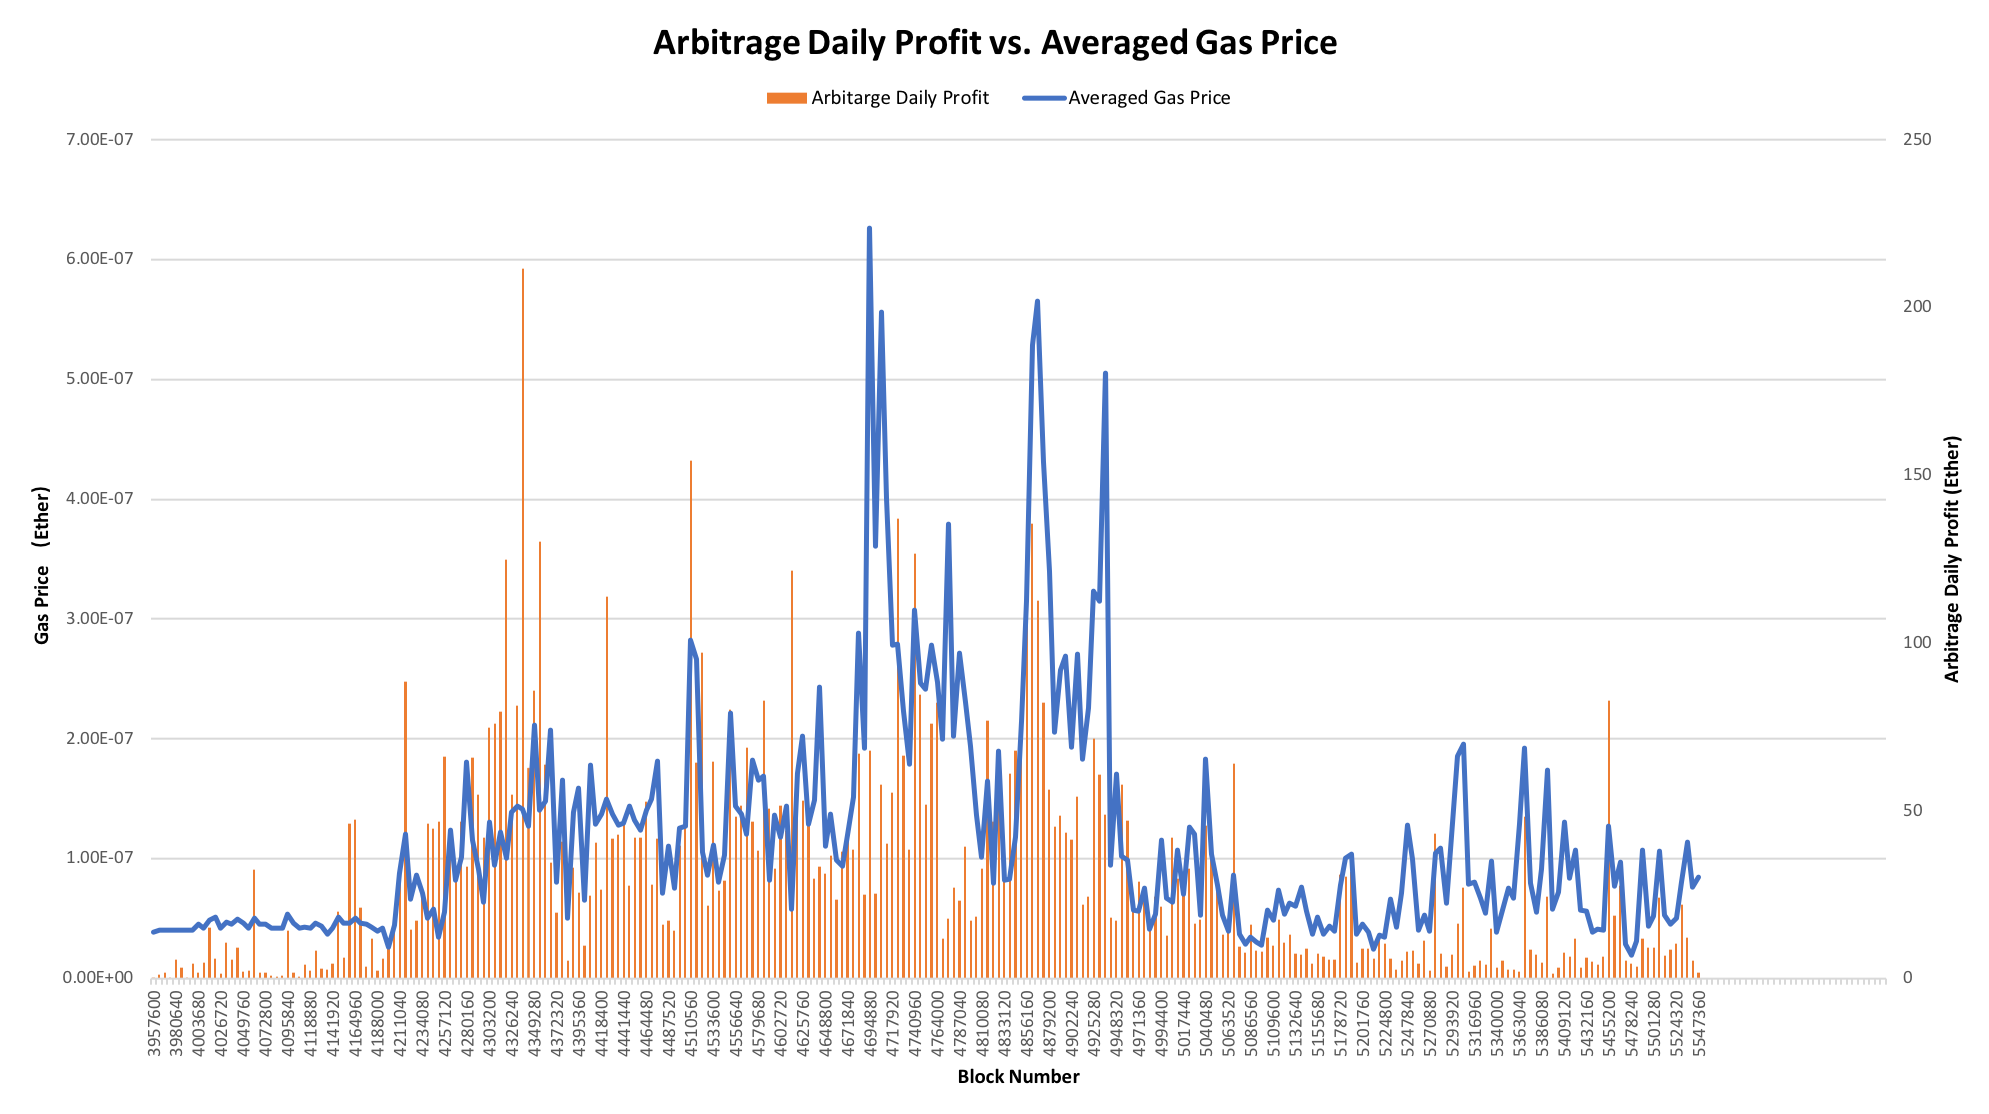
\includegraphics[width=0.5\textwidth]{figures/arb_daily_profit_vs_ave_gas_price.png}
    \item Are miners collaborating with arbitrageurs?\\
    Miners may not collaborate with arbitrageurs:\\
    \url{https://docs.google.com/spreadsheets/d/1ed_PNnKLF5nWvips5exa9lbiNsDOfb4Yzw0-dpzR4T8/edit?usp=sharing}
    \item Is EtherDelta colluding with the dominant arbitrageur?
    \item Ask Chainalysis for data on arbitrageur
    \item What is EtherD
    elta’s profit and how does it compare with the dominant arbitrageur’s profits? (Note that EtherDelta could eliminate the biggest opportunities with a better user interface.)
    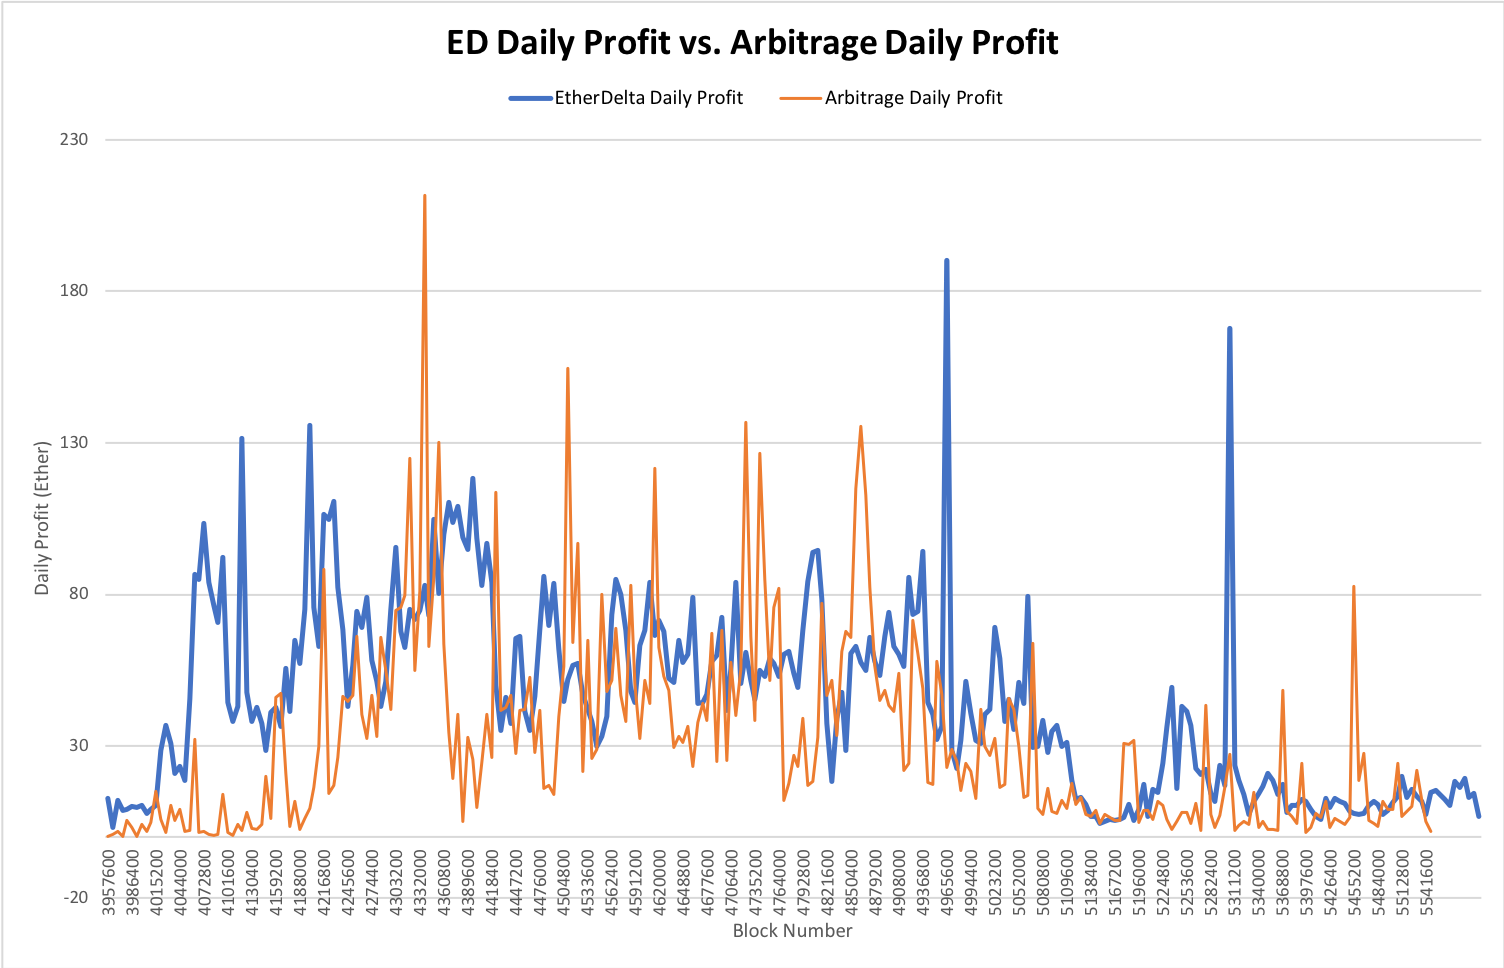
\includegraphics[width=0.5\textwidth]{figures/ed_arb_daily_profit.png}
    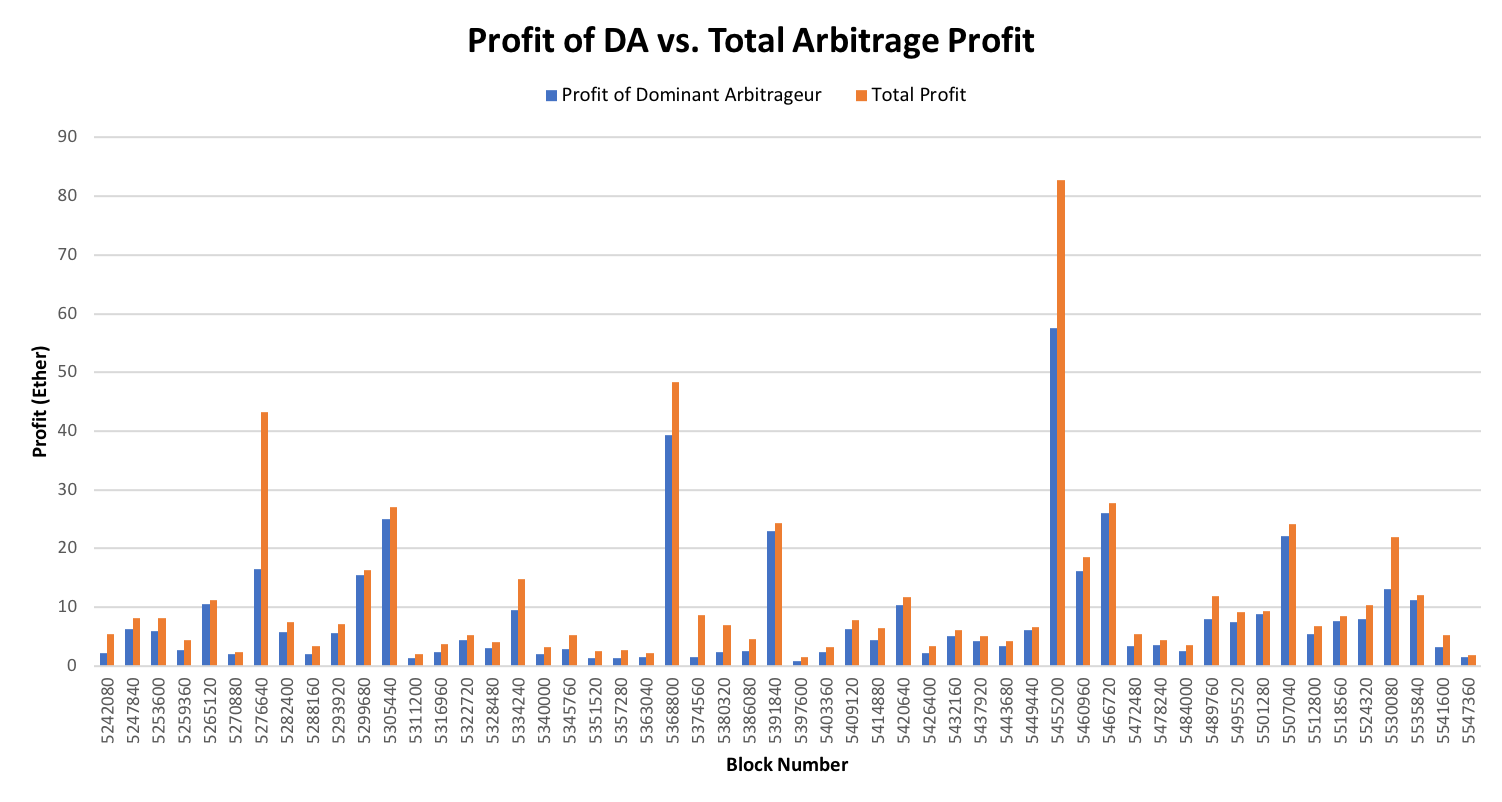
\includegraphics[width=0.5\textwidth]{figures/profit_da_vs_total.png}
    \item How to calculate the volume of arbitrage opportunities? (Relative to total trade volume as well)
    \item How did the dominant arbitrageur become dominant?
    
    \item How do new arbitrageurs enter and quit the market?
    
    From block 3900000(2017/6/30) to block 5550000(2018/5/4), there are 432 contracts with successful EtherDelta Trade, 272 of them have arbitrage transactions. 
    The arbitrageurs update their contracts sometimes. We merged those contracts that share one or more common administrators. There are 84 disjoint sets after the merge, so we assume there are 84 arbitrageurs during this period of time. (However, it is still possible the same arbitrageur publish his or her new contract with a completely new address.)
    Here is a figure showing the number of active arbitrageurs by time. There is a sharp increase in the beginning of Sept. 2017, after the blog post.
    
    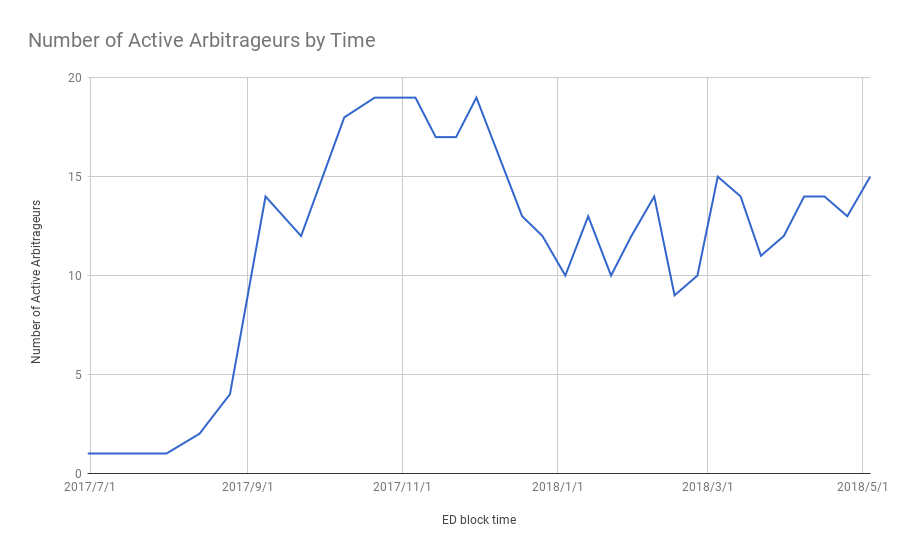
\includegraphics[width=0.5\textwidth]{figures/number_of_active_arbitrageurs_by_time.png}
    
    Another figure showing the length of active time period of each arbitrageur. We are investigating whether they lost money.
    
    
    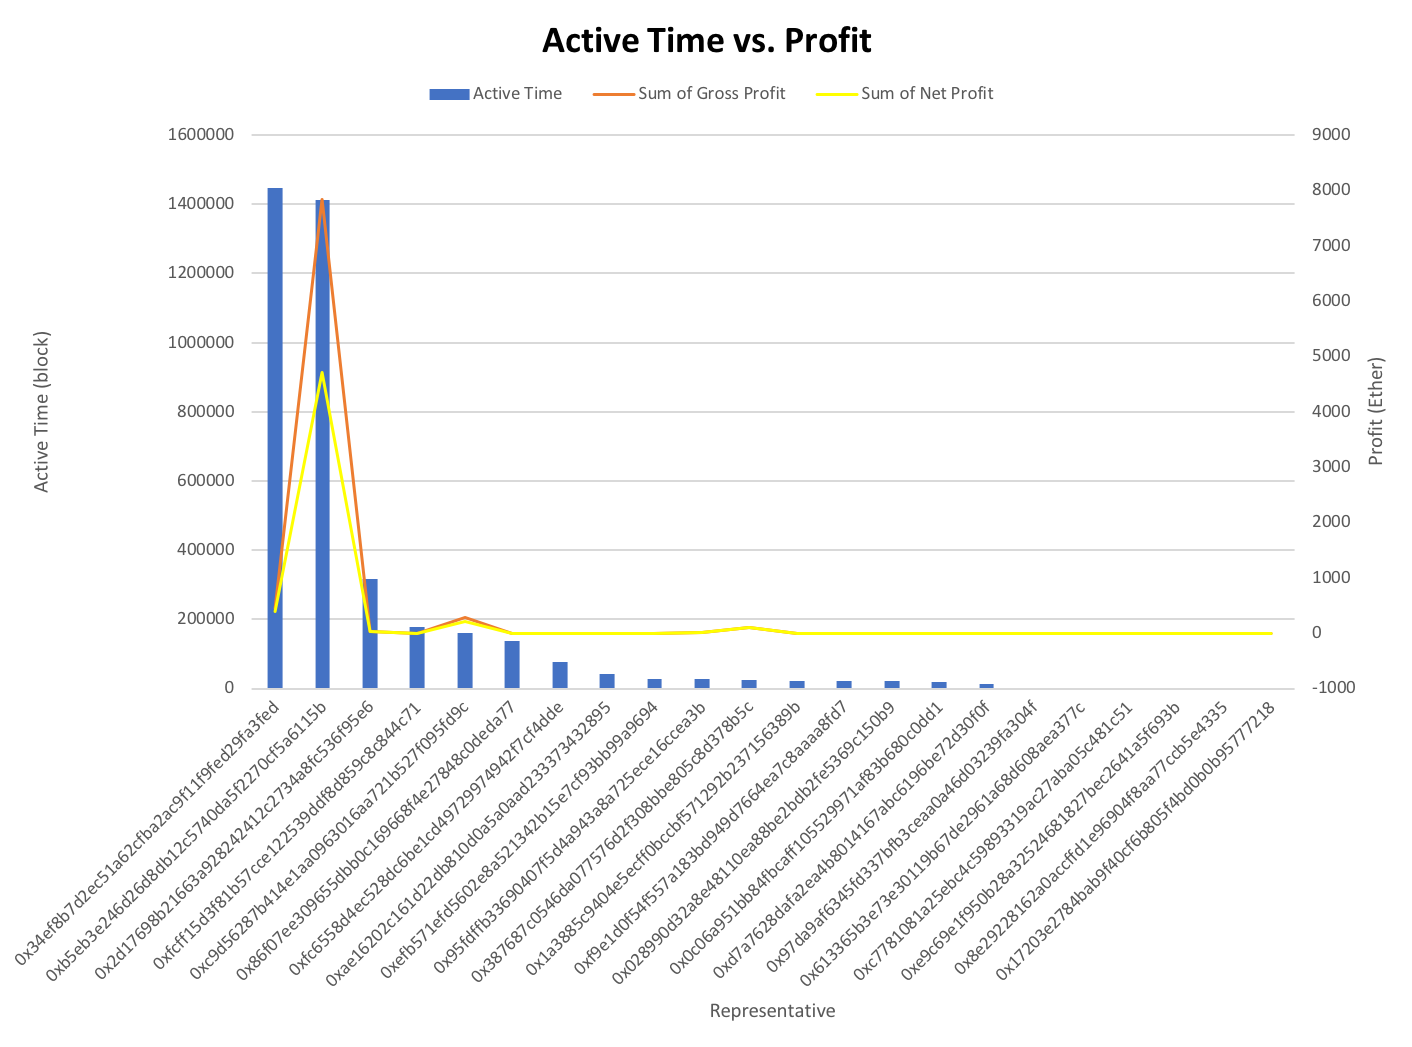
\includegraphics[width=0.5\textwidth]{figures/active_time_vs_profit.png}
    
    \item How did their strategies evolve?
    
    \item How frequently did arbitrageurs update their contracts? 
    \item How quickly did GasToken penetrate the market?
    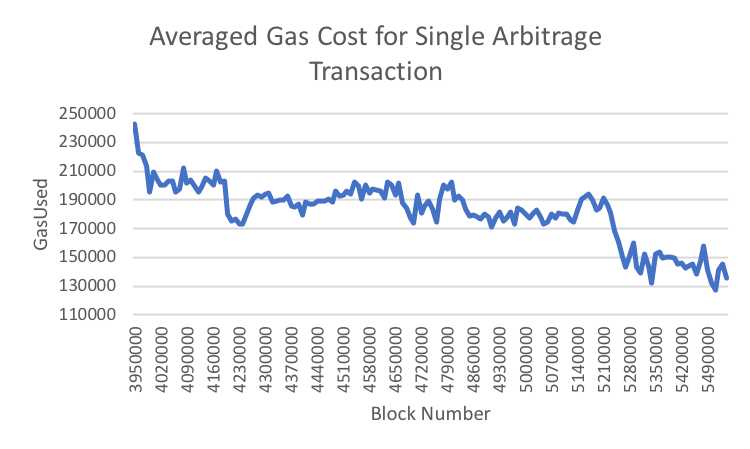
\includegraphics[width=0.5\textwidth]{figures/gasused.png}
    \item How to optimize the exchange to prevent the arbitrage from happening?
        
        EtherDelta webpage will alert the user when the buy order price is significantly higher than the best sell order price or the sell order price is significantly lower than the best buy order price.
when generating buy order:
\begin{verbatim}
    0 !== price && price > 1.5 * bestSell
\end{verbatim}

when generating sell order 
\begin{verbatim}
    0 !== price && "" !== price && price < .5 * bestBuy
\end{verbatim}


\end{itemize}
\section{Data}
\begin{itemize}
    \item Some initial results about the total arbitrage opportunity and its distribution:\\ \url{https://docs.google.com/document/d/16slmicyxrv77g3rJrH6jaxwZqYrjy4uXNWvodlBuVxY/edit?usp=sharing}
    \item Some statistics about the arbitrageurs' profit at different times:\\
    \url{https://docs.google.com/document/d/1TwI-MFxMCBXwI9701IrbZFUg9-PtWugMoucgz3alPAc/edit?usp=sharing}
    \item Raw data on lederhosen: 
    \begin{verbatim}
        /home/etherdelta_attack/stat_results
    \end{verbatim}
    There is also a short readme.txt in it.
\end{itemize}



\printbibliography



\end{document}
